\centering
$\mathrm{T}$ isosurfaces
\vskip-2ex
\rule{0.875\textwidth}{1pt}
\par

\begin{columns}[T]

  \begin{column}{0.02\textwidth}
  \end{column}

  \begin{column}{0.32\textwidth}
    \begin{figure}[H]
	    \begin{tikzpicture}
		    \node (isoC11Ro3Ra8) at (0,0) {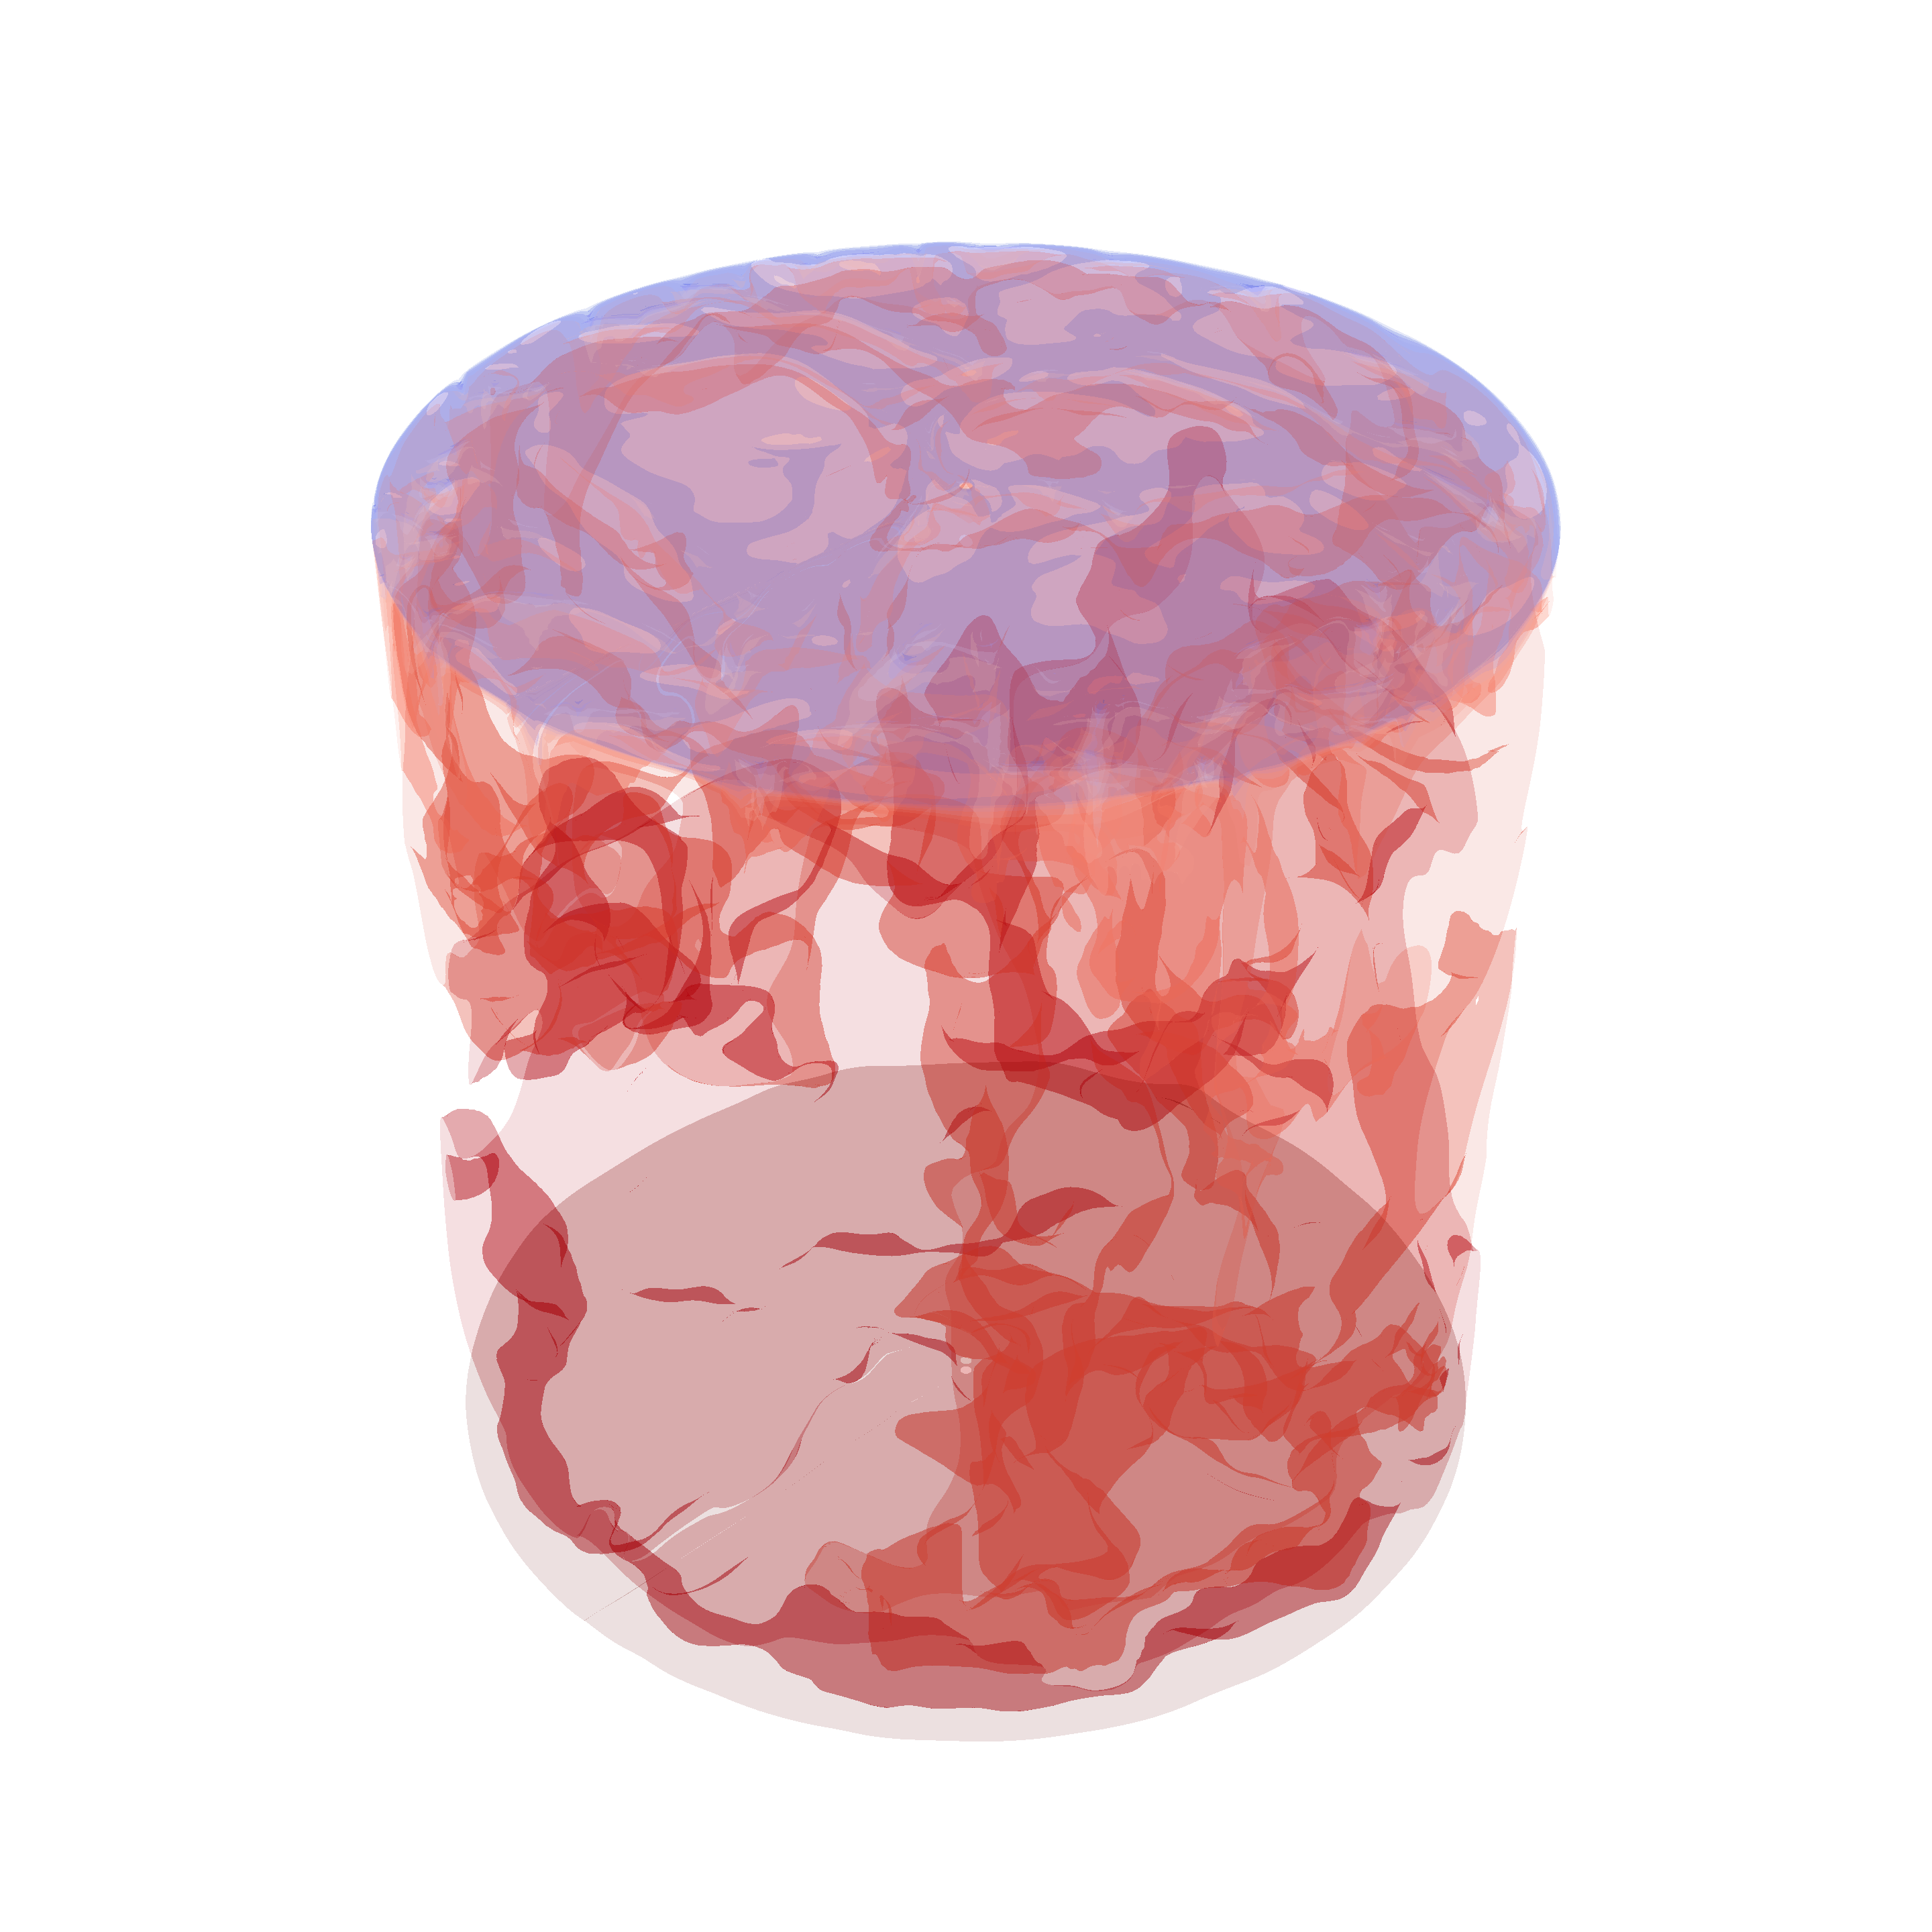
\includegraphics[width=\textwidth, trim={0 11cm 0 9cm},clip]{figs/isosurface_C11_Ro3_Ra10e8.png}};
		    \node [rectangle, fill=white, align=center] (isoTitle) at (isoC11Ro3Ra8.north) {\small \texttt{C1}, $\mathrm{Ra_m} = 10^8$, $\mathrm{Ro_m} = 3.0$};
	    \end{tikzpicture}
    \end{figure}
  \end{column}

  \begin{column}{0.32\textwidth}
    \begin{figure}[H]
	    \begin{tikzpicture}
		    \node (isoC11Ro1Ra8) at (0,0) {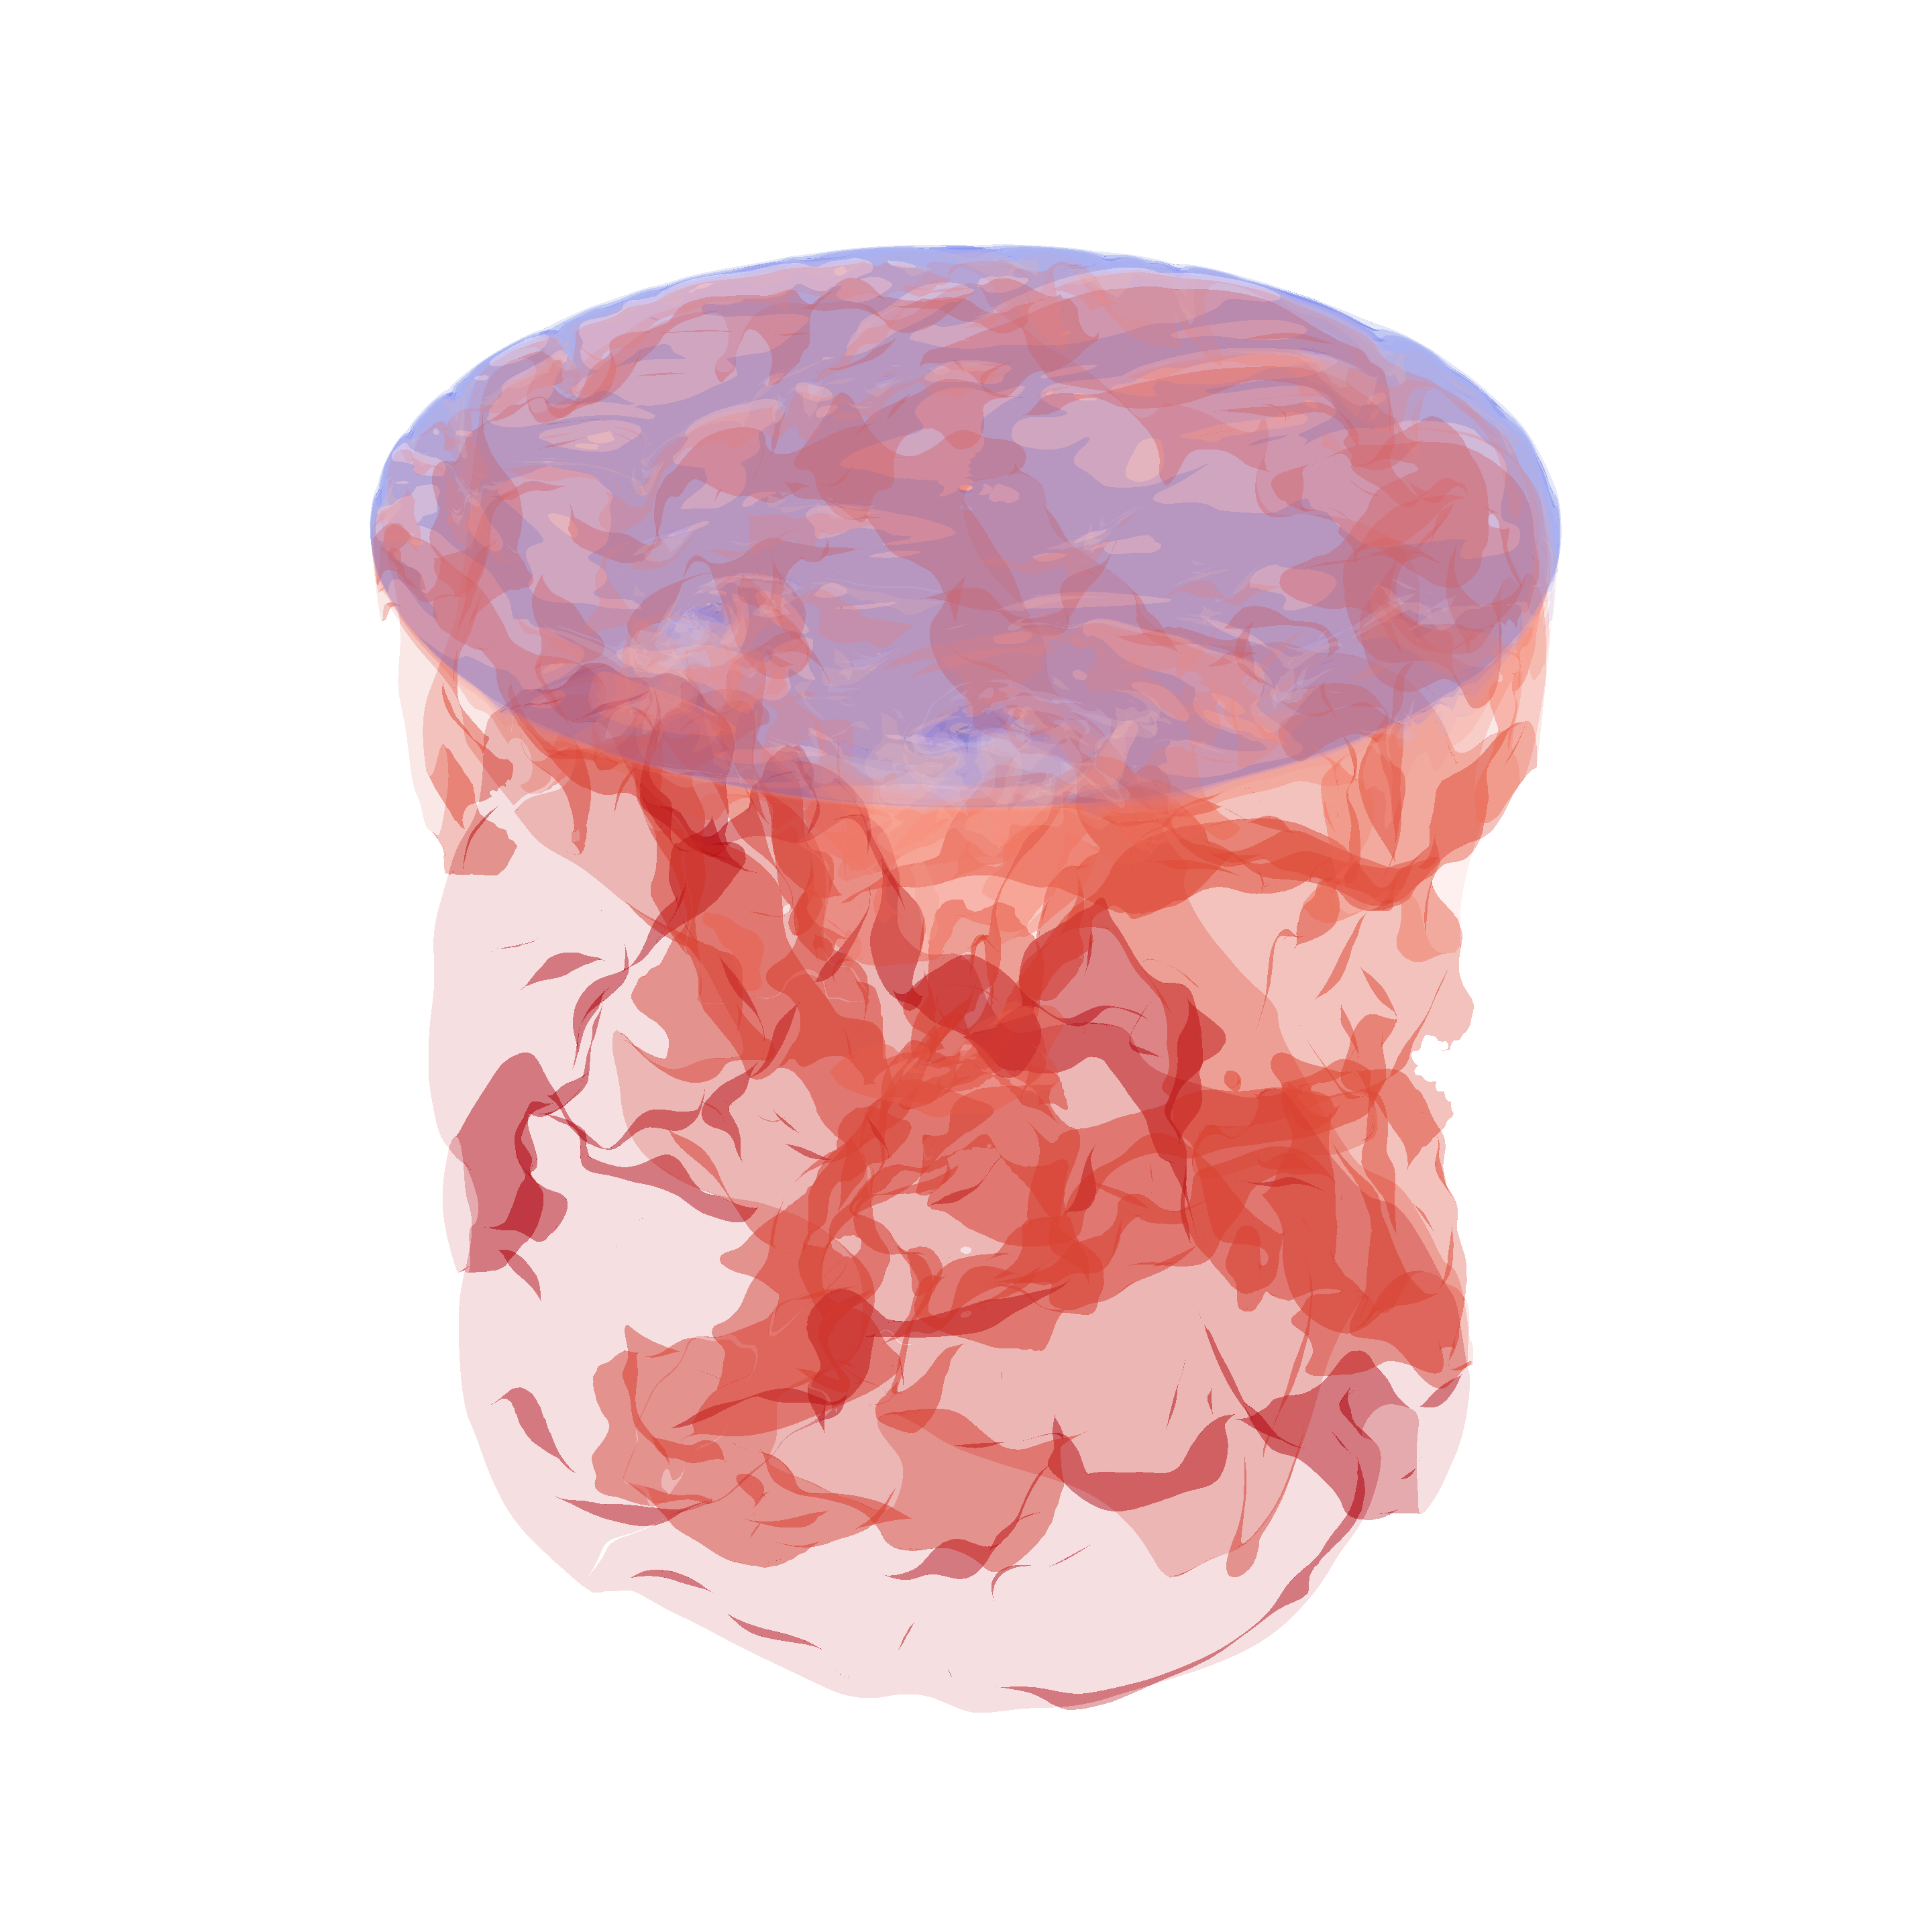
\includegraphics[width=\textwidth, trim={0 11cm 0 9cm},clip]{figs/isosurface_C11_Ro1_Ra10e8.png}};
		    \node [rectangle, fill=white, align=center] (isoTitle) at (isoC11Ro1Ra8.north) {\small \texttt{C1}, $\mathrm{Ra_m} = 10^8$, $\mathrm{Ro_m} = 1.0$};
		    \node (cbar) at ([yshift=-0.5cm]isoC11Ro1Ra8.south) {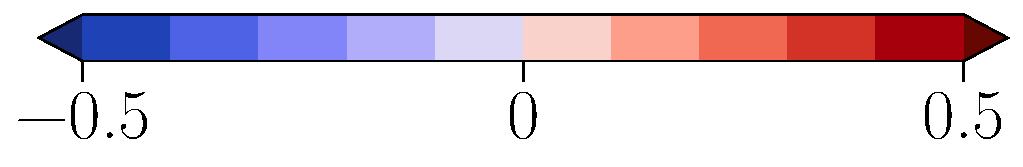
\includegraphics[width=0.75\textwidth]{figs/cbar.pdf}};
	    \end{tikzpicture}
%      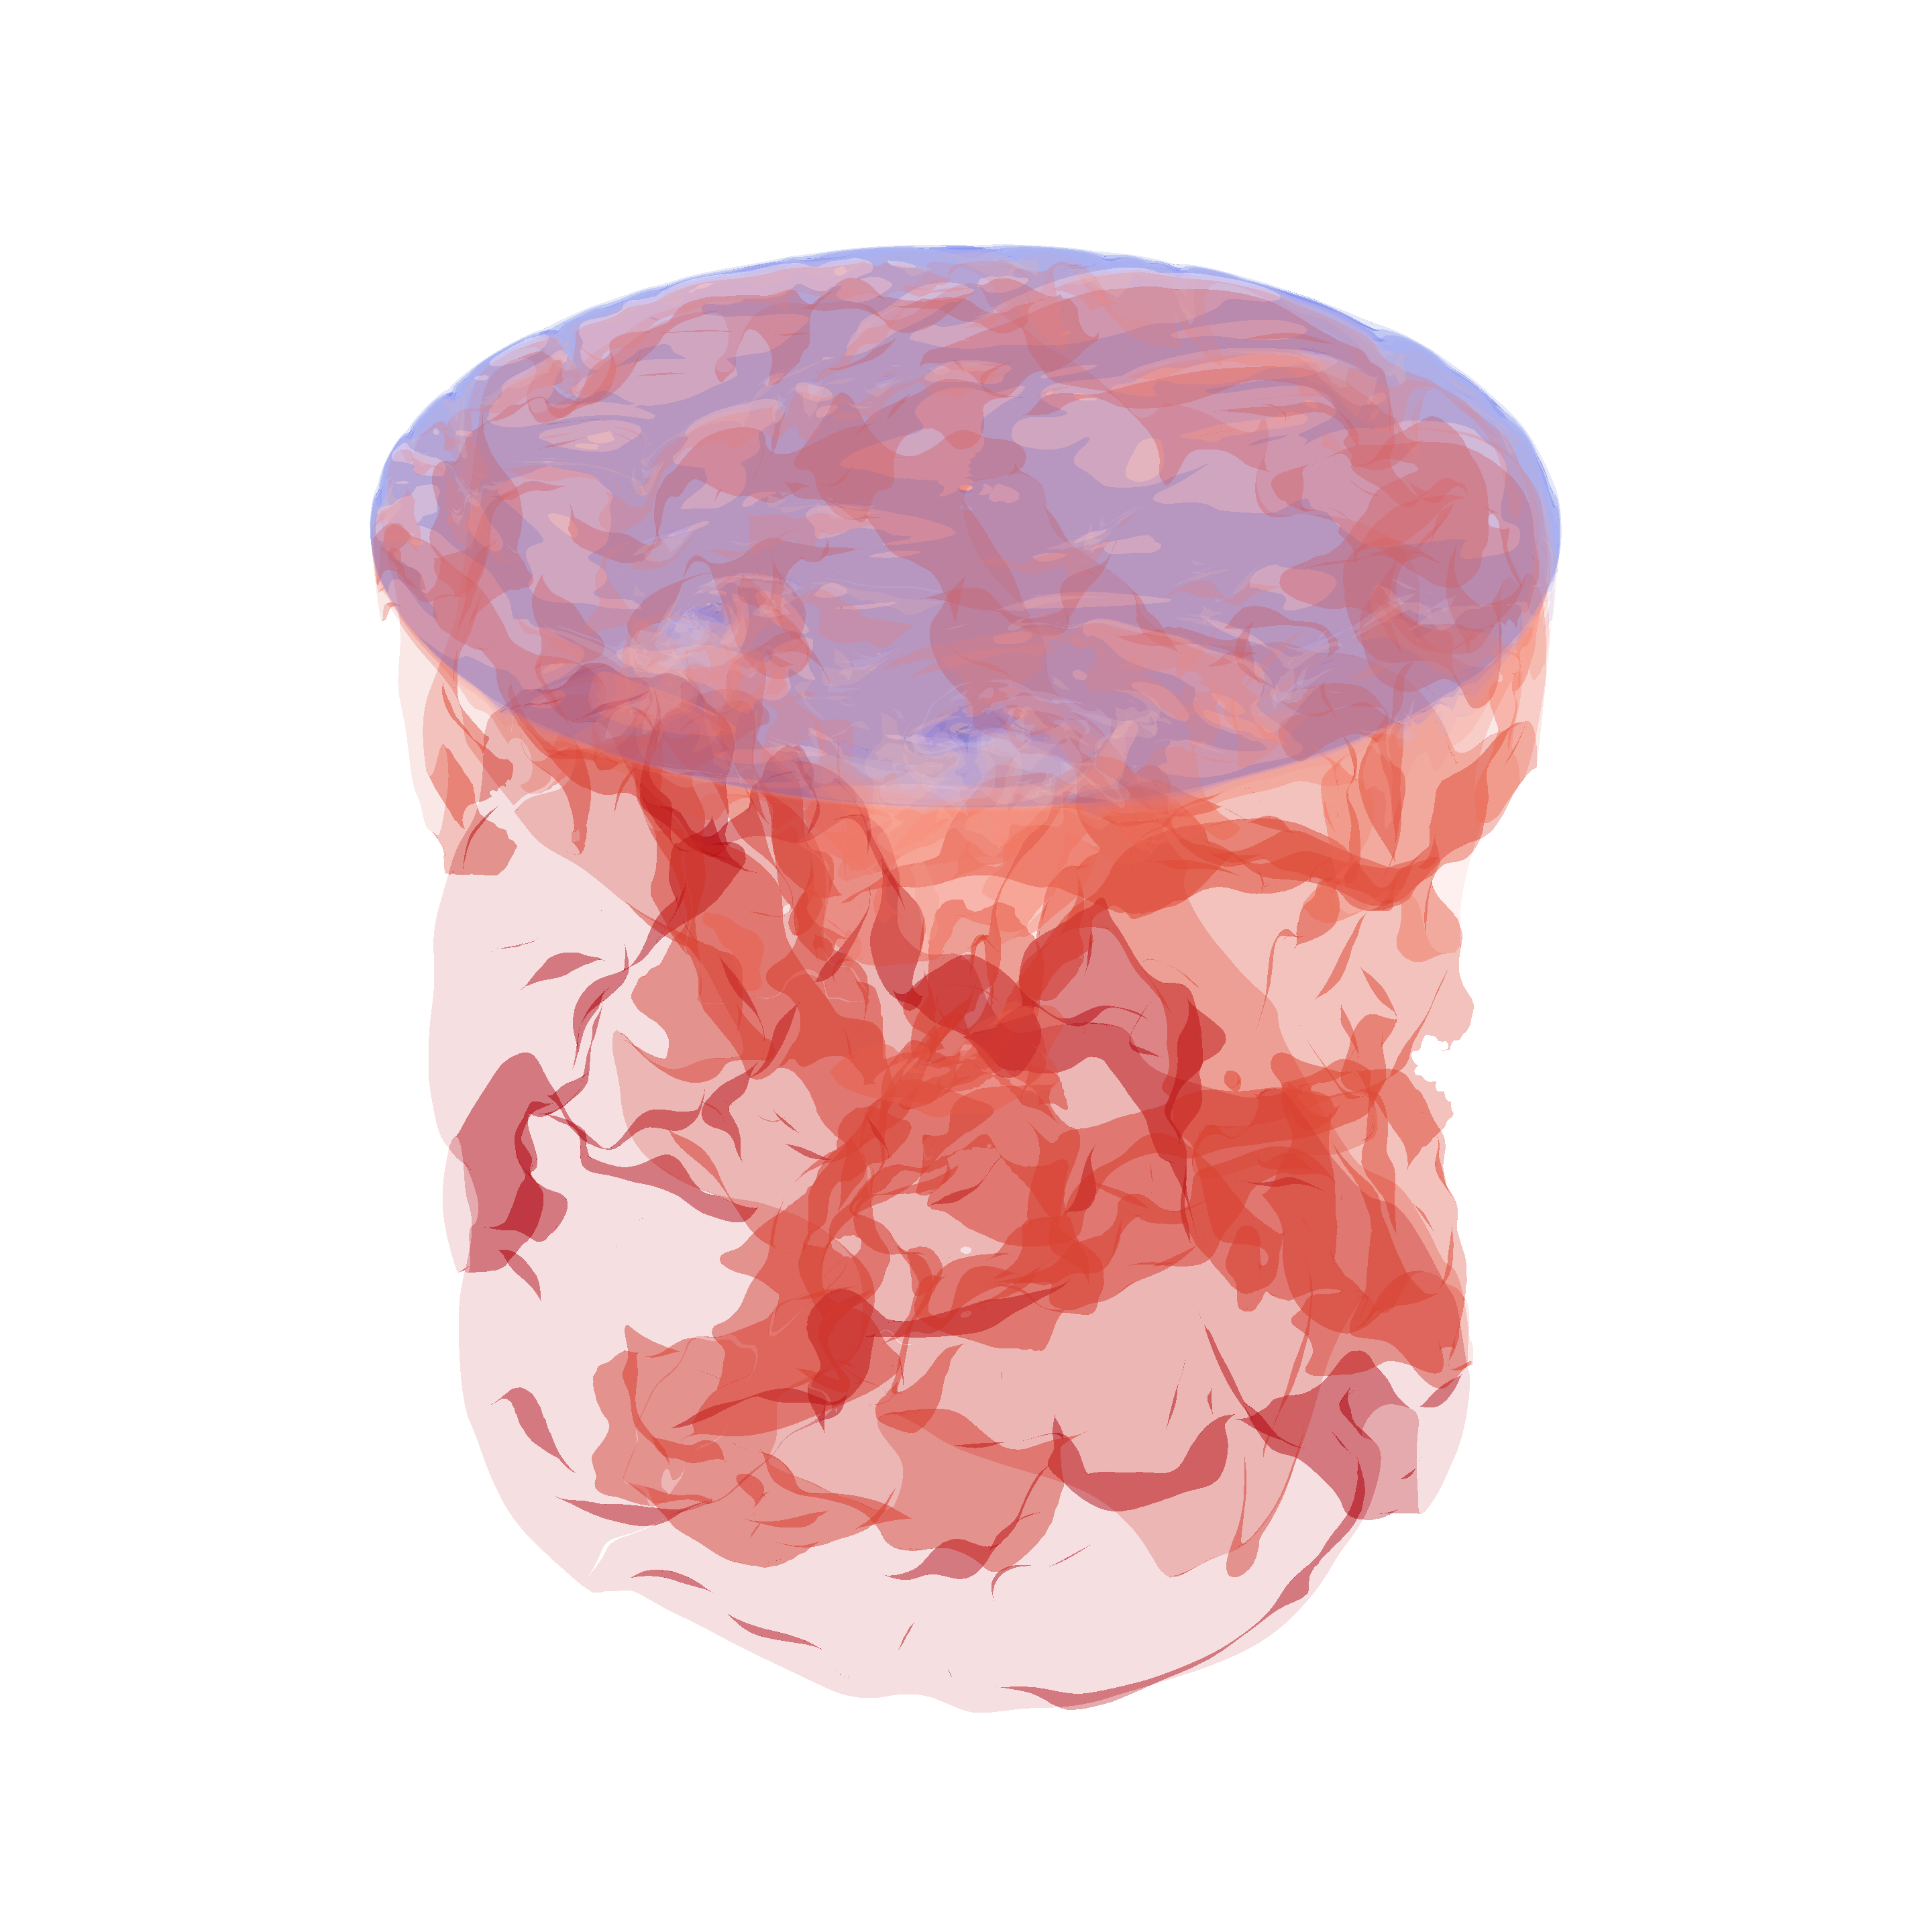
\includegraphics[width=\textwidth]{figs/isosurface_C11_Ro1_Ra10e8.png}
    \end{figure}
  \end{column}

  \begin{column}{0.32\textwidth}
    \begin{figure}[H]
	    \begin{tikzpicture}
		    \node (isoC11Ro02Ra8) at (0,0) {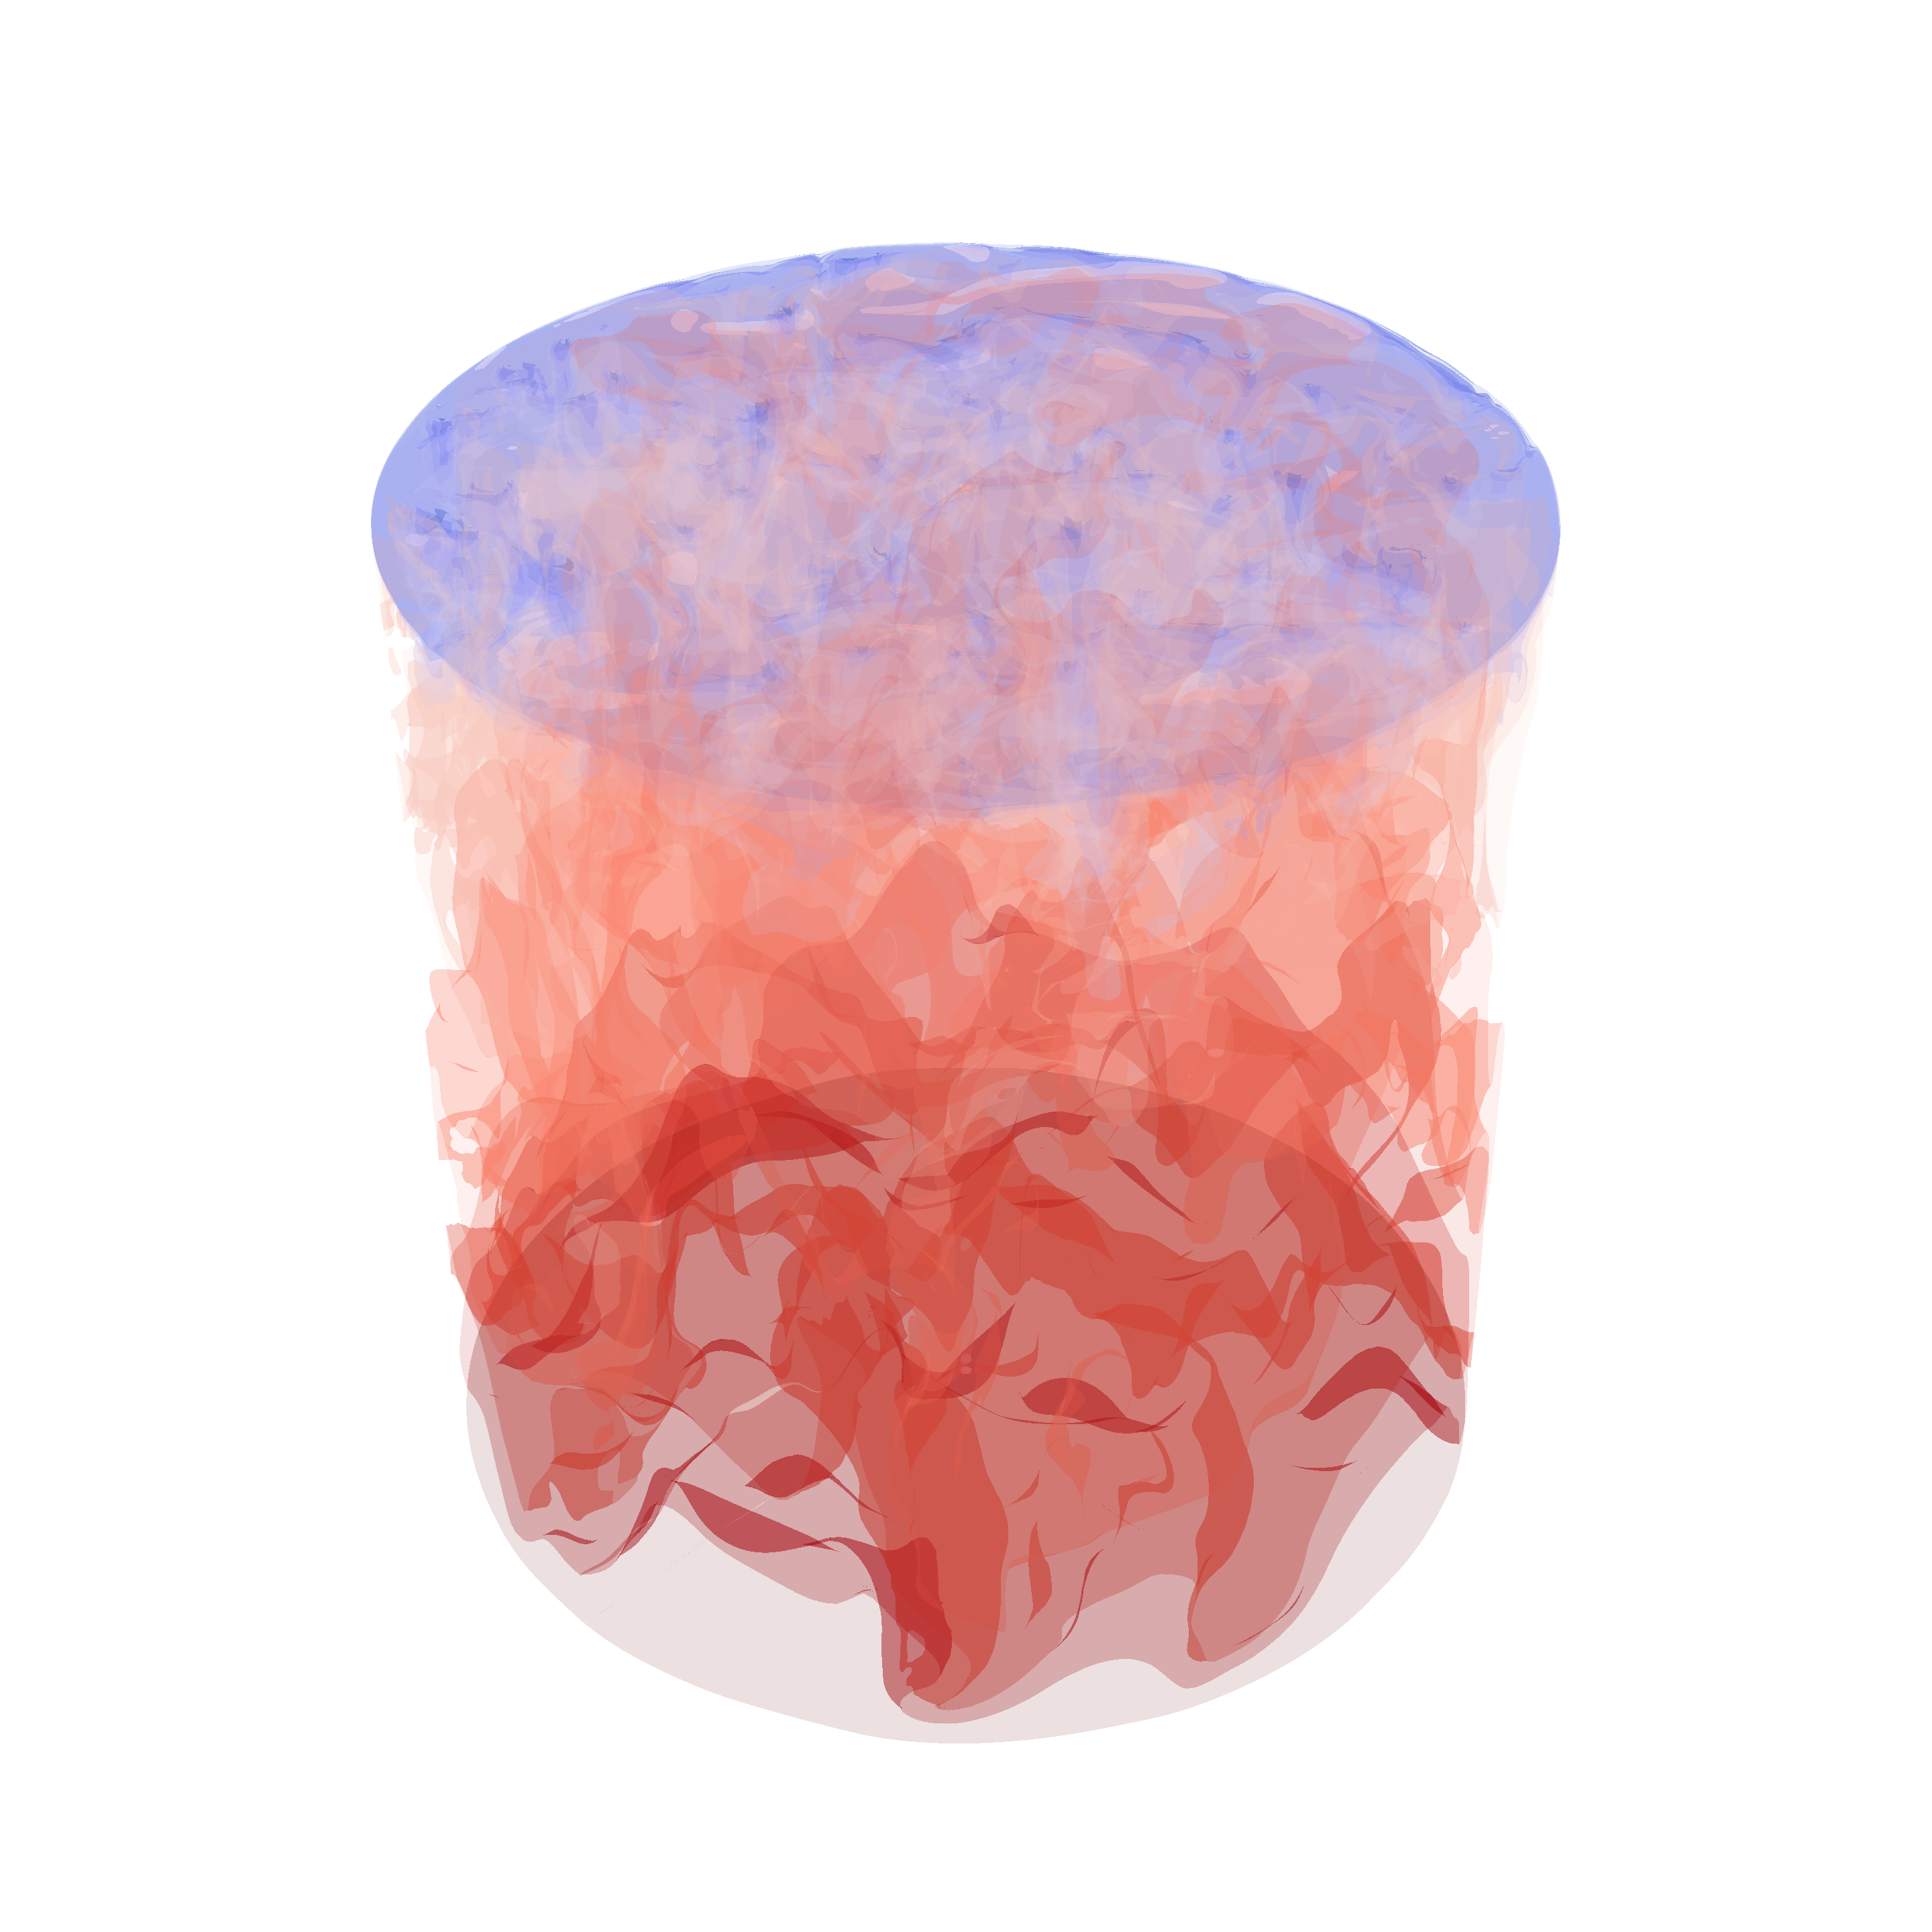
\includegraphics[width=\textwidth, trim={0 11cm 0 9cm},clip]{figs/isosurface_C11_Ro02_Ra10e8.png}};
		    \node [rectangle, fill=white, align=center] (isoTitle) at (isoC11Ro02Ra8.north) {\small \texttt{C1}, $\mathrm{Ra_m} = 10^8$, $\mathrm{Ro_m} = 0.2$};
	    \end{tikzpicture}
%      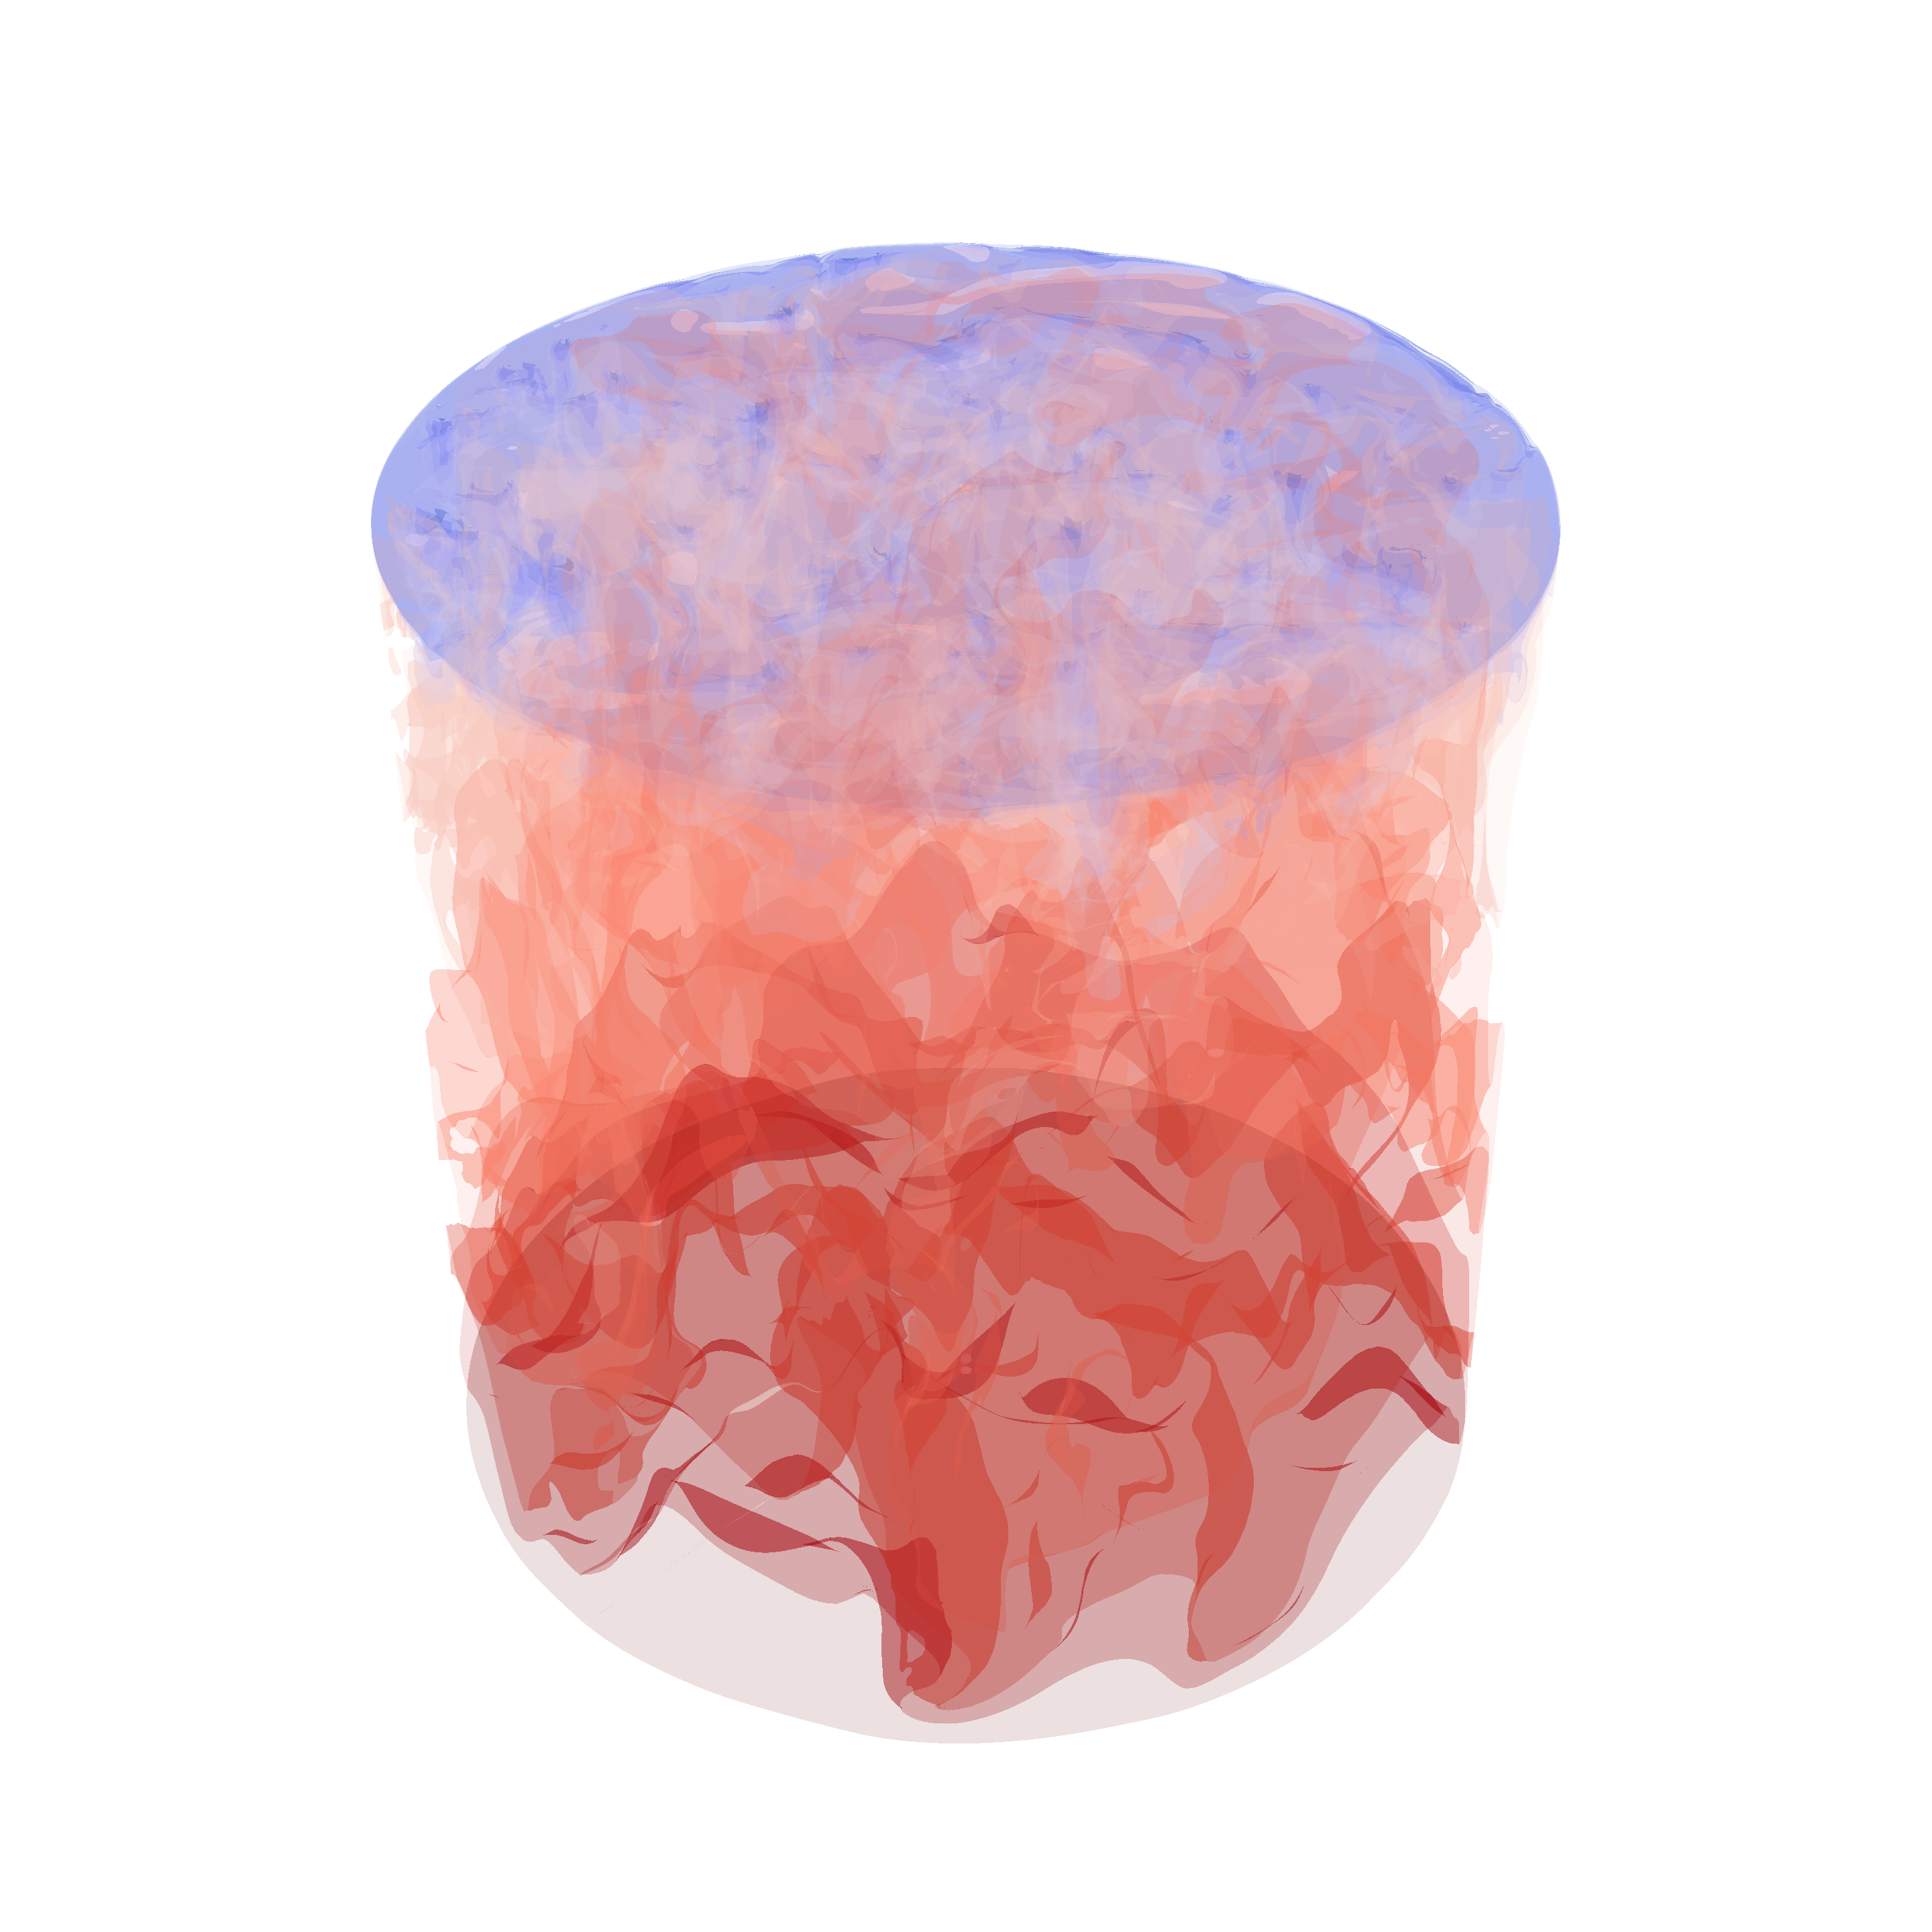
\includegraphics[width=\textwidth]{figs/isosurface_C11_Ro02_Ra10e8.png}
    \end{figure}
  \end{column}

  \begin{column}{0.02\textwidth}
  \end{column}
\end{columns}
\begin{outline}
	\1 As rotation rate increases (i.e. $Ro_m$ decreases), the supercriticalities decreases. 
	\1 Case $C1$ at $Ro_m = 1.0$, $3.0$ and $Ra_m=10^8$ still permits all three types of convection to occur. 
	\1 For case $C1$ at $Ro_m = 0.2$ and $Ra_m=10^8$, stationary convection is prohibited at approximately $T \geq 0.3$, thus oscillatory convection dominates.

\end{outline}
\centering
$\mathbf{u_z}$ isosurfaces
\vskip-2ex
\rule{0.875\textwidth}{1pt}
\par
\begin{columns}[T]

  \begin{column}{0.02\textwidth}
  \end{column}

  \begin{column}{0.32\textwidth}
    \begin{figure}[H]
	    \begin{tikzpicture}
		    \node (uzisoC11Ro3Ra8) at (0,0) {\includegraphics[width=\textwidth, trim={0 15cm 0 15cm},clip]{figs/isosurface_C11_Ro3_Ra10e8xy.png}};
		    \node [rectangle, fill=white, align=center] (Title) at (uzisoC11Ro3Ra8.north) {\small \texttt{C1}, $\mathrm{Ra_m} = 10^8$, $\mathrm{Ro_m} = 3.0$};
	    \end{tikzpicture}
%      \includegraphics[width=\textwidth]{figs/isosurface_C11_Ro02_Ra10e6.png}
    \end{figure}
  \end{column}

  \begin{column}{0.32\textwidth}
    \begin{figure}[H]
	    \begin{tikzpicture}
		    \node (uzisoC11Ro1Ra8) at (0,0) {\includegraphics[width=\textwidth, trim={0 15cm 0 15cm},clip]{figs/isosurface_C11_Ro1_Ra10e8xy.png}};
		    \node [rectangle, fill=white, align=center] (Title) at (uzisoC11Ro1Ra8.north) {\small \texttt{C1}, $\mathrm{Ra_m} = 10^8$, $\mathrm{Ro_m} = 1.0$};
		    \node (cbar) at ([yshift=-0.5cm]uzisoC11Ro1Ra8.south) {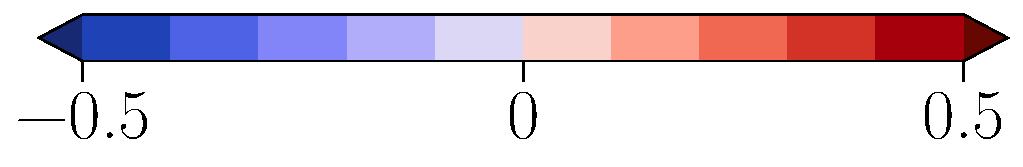
\includegraphics[width=0.75\textwidth]{figs/cbar.pdf}};
	    \end{tikzpicture}
%      \includegraphics[width=\textwidth]{figs/isosurface_C11_Ro02_Ra10e6.png}
    \end{figure}
  \end{column}

  \begin{column}{0.32\textwidth}
    \begin{figure}[H]
	    \begin{tikzpicture}
		    \node (uzisoC11Ro02Ra8) at (0,0) {\includegraphics[width=\textwidth, trim={0 15cm 0 15cm},clip]{figs/isosurface_C11_Ro02_Ra10e8xy.png}};
		    \node [rectangle, fill=white, align=center] (Title) at (uzisoC11Ro02Ra8.north) {\small \texttt{C1}, $\mathrm{Ra_m} = 10^8$, $\mathrm{Ro_m} = 0.2$};
	    \end{tikzpicture}
%      \includegraphics[width=\textwidth]{figs/isosurface_C11_Ro02_Ra10e7.png}
    \end{figure}
  \end{column}

  \begin{column}{0.02\textwidth}
  \end{column}
  \end{columns}
\centering
Flow statistics
\vskip-2ex
\rule{0.875\textwidth}{1pt}
\par
\begin{columns}[T]

  \begin{column}{0.02\textwidth}
  \end{column}

  \begin{column}{0.32\textwidth}
    \begin{figure}[H]
	    \begin{tikzpicture}
	    \begin{axis}[
		width=0.75\textwidth, % Match figure width
		height=0.75\textwidth, % Adjust height as needed
		enlargelimits=false, % Keep exact figure limits
		    title={\small Conductive temperature profile},
		title style={align=center, yshift=-0.5ex , text width=0.75\textwidth},
		xmin=-0.5, xmax=0.5, % Adjust based on your data
		ymin=0, ymax=1, % Adjust based on your data
		axis line style={draw=none}, % Remove axis border
		tick style={draw=none}, % Hide tick marks
		ticks=none, % Hide default ticks
		clip=false, % Prevent clipping of labels
		every axis background/.style={fill=white} % Keep fill colo
	    ]
	    \addplot graphics[xmin=-0.5, xmax=0.5, ymin=0, ymax=1] {figs/Tcond.pdf};
	    \end{axis}
	\end{tikzpicture}
    \end{figure}
  \end{column}

  \begin{column}{0.32\textwidth}
    \begin{figure}[H]
	    \begin{tikzpicture}
	    \begin{axis}[
		width=0.75\textwidth, % Match figure width
		height=0.75\textwidth, % Adjust height as needed
		enlargelimits=false, % Keep exact figure limits
		    title={\small Mean temperature profile},
		title style={align=center, yshift=-0.5ex , text width=0.75\textwidth},
		xmin=-0.5, xmax=0.5, % Adjust based on your data
		ymin=0, ymax=1, % Adjust based on your data
		axis line style={draw=none}, % Remove axis border
		tick style={draw=none}, % Hide tick marks
		ticks=none, % Hide default ticks
		clip=false, % Prevent clipping of labels
		every axis background/.style={fill=white} % Keep fill colo
	    ]
	    \addplot graphics[xmin=-0.5, xmax=0.5, ymin=0, ymax=1] {figs/z_T_mean.pdf};
	    \end{axis}
	\end{tikzpicture}
    \end{figure}
  \end{column}

  \begin{column}{0.32\textwidth}
    \begin{figure}[H]
	    \begin{tikzpicture}
	    \begin{axis}[
		width=0.75\textwidth, % Match figure width
		height=0.75\textwidth, % Adjust height as needed
		enlargelimits=false, % Keep exact figure limits
		    title={\small Mean temperature deviation },
		title style={align=center, yshift=-0.5ex, text width=0.75\textwidth},
		xmin=-0.5, xmax=0.5, % Adjust based on your data
		ymin=0, ymax=1, % Adjust based on your data
		axis line style={draw=none}, % Remove axis border
		tick style={draw=none}, % Hide tick marks
		ticks=none, % Hide default ticks
		clip=false, % Prevent clipping of labels
		every axis background/.style={fill=white} % Keep fill colo
	    ]
	    \addplot graphics[xmin=-0.5, xmax=0.5, ymin=0, ymax=1] {figs/z_T_mean_noCOnd.pdf};
	    \end{axis}
	    \end{tikzpicture}
    \end{figure}
  \end{column}

  \begin{column}{0.02\textwidth}
  \end{column}
\end{columns}
\begin{outline}
	\1 Flow results show strong NOB characteristics as the fluid has a much higher $T_c - T_{m}$. 
	\1 Rotation is observed to suppress NOB effects, as the rapidly-rotating cases ($Ro_m=0.2$) show a much lower $T_c - T_m$ that the slowly-rotating cases ($Ro_m=1.0$, $3.0$). 
	\1 These results were also observed in \cite{Horn2014}.
\end{outline}

